\subsection{Понятие предела функции многих переменных} \label{sec:1.3}
\begin{tbox}{Предел функции одной переменной}
	Вспомним определение предела для функции одной действительной переменной. Пусть \( y = f(x) \), где \( x \in \mathbb{E} \subset \mathbb{R} \). Точка \( x = a \) является предельной точкой множества \( \mathbb{E} \); она может как принадлежать \( \mathbb{E} \), так и не принадлежать ему (\( a \in \mathbb{E} \) или \( a \notin \mathbb{E} \)).

	\begin{multline} \label{eq:1.3.1}
		\lim_{x \to a} f(x) = A \Leftrightarrow
		(\forall \varepsilon > 0) \, (\exists \delta = \delta(\varepsilon) > 0) \,
		(\forall x \in \mathbb{E}, \, 0 < |x - a| < \delta) : \\
		|f(x) - A| < \varepsilon
	\end{multline}

	В определении предела неравенство \( 0 < |x - a| < \delta \) означает, что \( x \in (a - \delta, a + \delta) \) и \( x \neq a \). Геометрический смысл модуля \( |x - a| = \rho(x, a) \) — это расстояние между точками \( x \) и \( a \) на действительной оси, причём \( 0 < \rho(x, a) < \delta \).
\end{tbox}

\begin{tbox}{Предел функции многих переменных}
	Обобщим определение предела на случай функции многих переменных. Пусть \( y = f(\vec{x}) = f(x_1, x_2, \dots, x_k) \) определена на множестве \( \mathbb{E} \subset \mathbb{R}^k \). Точка \( \vec{a} = (a_1, a_2, \dots, a_k) \) является предельной для \( \mathbb{E} \) и может как принадлежать \( \mathbb{E} \), так и не принадлежать ему (\( \vec{a} \in \mathbb{E} \) или \( \vec{a} \notin \mathbb{E} \)).

	Расстояние между точками в \( \mathbb{R}^k \) было введено в \cref{sec:1.1}:
	\begin{align}
		\rho(\vec{x}, \vec{a}) = \|\vec{x} - \vec{a}\| =
		\sqrt{(x_1 - a_1)^2 + (x_2 - a_2)^2 + \dots + (x_k - a_k)^2}.
	\end{align}

	Предел функции многих переменных обозначается следующим образом:
	\begin{align}
		\lim_{\vec{x} \to \vec{a}} f(\vec{x}) = A \quad \text{или} \quad
		\lim_{\substack{x_1 \to a_1 \\ x_2 \to a_2 \\ \vdots \\ x_k \to a_k}}
		f(x_1, x_2, \dots, x_k) = A.
	\end{align}

	На языке «\(\varepsilon\)-\(\delta\)» определение аналогично \cref{eq:1.3.1}, но вместо чисел \( x \) и \( a \) используются векторы \( \vec{x} \) и \( \vec{a} \), а модуль \( |x - a| \) заменяется на норму \( \|\vec{x} - \vec{a}\| \):
	\begin{align}
		(\forall \varepsilon > 0) \, (\exists \delta = \delta(\varepsilon) > 0) \,
		(\forall \vec{x} \in \mathbb{E}, \, 0 < \|\vec{x} - \vec{a}\| < \delta) :
		|f(\vec{x}) - A| < \varepsilon
		\label{eq:2}
	\end{align}
\end{tbox}

\begin{tbox*}{Замечание о пределах}
	\textbf{Замечание.} Поскольку определение предела \eqref{eq:2} для функции многих переменных совпадает с определением для функции одной переменной, все теоремы о пределах, доказанные для случая одной переменной, переносятся на случай многих переменных.
\end{tbox*}

\begin{tbox}{Двойной предел}
	Рассмотрим предел функции двух переменных \( z = f(x, y) \), называемый двойным пределом. Пусть точка \( M(x, y) \in \mathbb{E} \subset \mathbb{R}^2 \) принадлежит области определения функции, а точка \( M_0(a, b) \) является предельной для \( \mathbb{E} \) (\( M_0 \in \mathbb{E} \) или \( M_0 \notin \mathbb{E} \)). Тогда:
	\begin{align}
		A = \lim_{M \to M_0} f(x, y) =
		\lim_{\substack{x \to a \\ y \to b}} f(x, y).
	\end{align}

	Расстояние между точками \( M \) и \( M_0 \) вычисляется по формуле:
	\[
	\rho(M, M_0) = \sqrt{(x - a)^2 + (y - b)^2} < \delta.
	\]

	На языке «\(\varepsilon\)-\(\delta\)» двойной предел записывается так:
	\begin{align}
		(\forall \varepsilon > 0) \, (\exists \delta = \delta(\varepsilon) > 0) \,
		(\forall (x, y) \in \mathbb{E}, \, 0 < \sqrt{(x - a)^2 + (y - b)^2} < \delta) : \\
		|f(x, y) - A| < \varepsilon
		\label{eq:3}
	\end{align}
\end{tbox}
\begin{figure}[t]
	\centering
	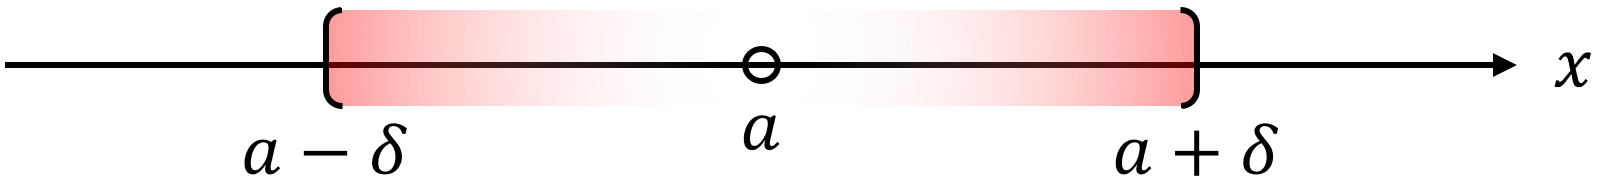
\includegraphics[width=0.7\linewidth]{image/screenshot008}
	\caption{Интервал $(a - \delta, a + \delta)$ с выколотой точкой}
	\label{fig:1.3.1}
\end{figure}
\begin{tbox}{Геометрический смысл двойного предела}
	Рассмотрим геометрический смысл неравенства:
	\begin{gather}
		0 < \sqrt{(x - a)^2 + (y - b)^2} < \delta = \delta(\varepsilon), \\
		0 < (x - a)^2 + (y - b)^2 < \delta^2(\varepsilon).
	\end{gather}

	Это задаёт круг радиуса \( \delta(\varepsilon) \) с выколотым центром в точке \( M_0(a, b) \). Такой круг называют \(\delta\)-окрестностью точки \( M_0 \) (\Cref{fig:1.3.2.1}).

	Для сравнения: в случае функции \( y = f(x) \) \(\delta\)-окрестность точки \( a \) — это интервал \( (a - \delta, a + \delta) \) с выколотой точкой \( a \) (\Cref{fig:1.3.1}).
\end{tbox}

\begin{tbox}{Независимость предела от пути}
	Из определения двойного предела следует, что если предел существует, то он не зависит от пути, по которому точка \( M \) приближается к \( M_0 \). Число возможных направлений бесконечно, в отличие от функции одной переменной, где таких направлений всего два (слева и справа от точки \( a \)).
\end{tbox}

\begin{figure}[H]
	\centering
	\begin{minipage}{0.45\linewidth}
		\centering
		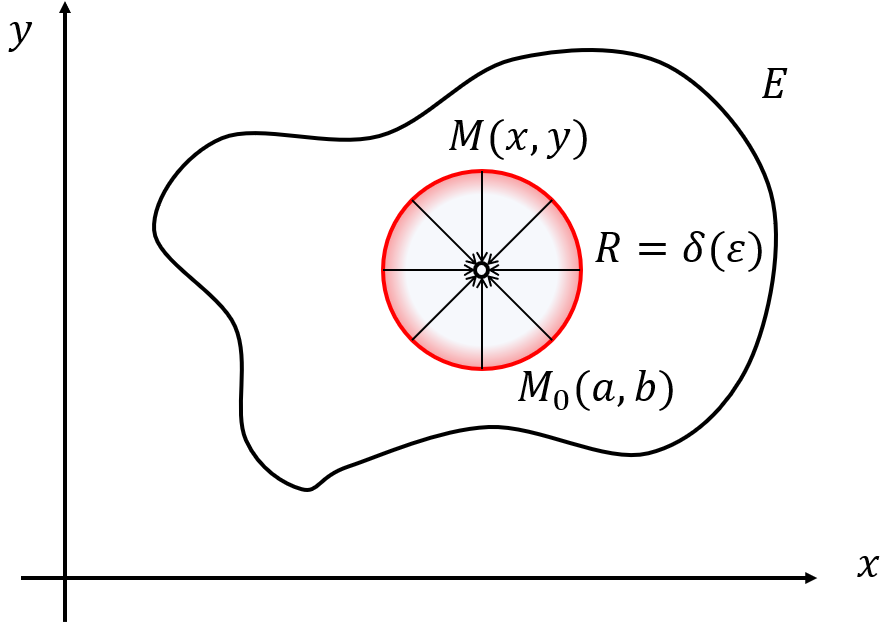
\includegraphics[width=0.9\linewidth]{image/screenshot009.png}
		\caption{ }
		\label{fig:1.3.2.1}
	\end{minipage}
	\begin{minipage}{0.45\linewidth}
		\centering
		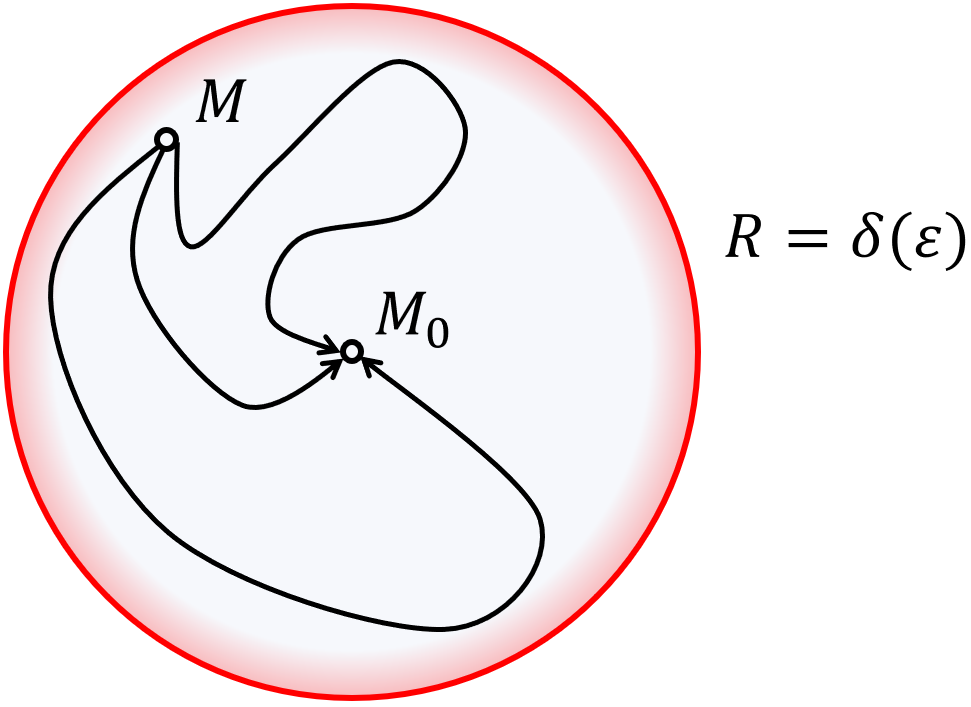
\includegraphics[width=0.9\linewidth]{image/screenshot010.png}
		\caption{ }
		\label{fig:1.3.2.2}
	\end{minipage}
\end{figure}

\subsubsection{Примеры решения двойных пределов}
\begin{enumerate}
	\item Вместо $x$ и $y$ подставляем предельные значения:
	\begin{align*}
		\lim_{\tiny{\begin{array}[b]{c} x \to 1\\y \to 2 \end{array}}} \frac{x \cdot y}{x^2 + y^2} =
		\frac{1 \cdot 2}{1^2 + 2^2} =
		\frac{2}{5}
	\end{align*}

	\item По теореме и произведении бесконечно малых на ограниченную:
	\begin{align*}
		\lim_{\tiny{\begin{array}[b]{c} x \to 0\\y \to 0 \end{array}}} (x + y \cdot \sin \frac{1}{x}) =
		\lim_{x \to 0} x + \lim_{\tiny{\begin{array}[b]{c} x \to 0\\y \to 0 \end{array}}} y \cdot \sin \frac{1}{x} =
		0
	\end{align*}

	\item Используя первый замечательный предел:
	\begin{multline*}
		\lim_{\tiny{\begin{array}[b]{c} x \to \infty \\y \to 2 \end{array}}} \left(x \cdot \sin \frac{1}{xy}\right) \, [\infty \cdot 0] =
		\lim_{\tiny{\begin{array}[b]{c} x \to \infty \\y \to 2 \end{array}}} \left(\frac{\sin \frac{1}{xy}}{\frac{1}{x}}\right) \left[\frac{0}{0}\right] =\\=
		\lim_{\tiny{\begin{array}[b]{c} x \to \infty \\y \to 2 \end{array}}} \left(\frac{\sin \frac{1}{xy}}{\frac{1}{xy} \cdot y}\right) =
		\lim_{y \to 2} \frac{1}{y} = \frac{1}{2}
	\end{multline*}

	\item Покажем что предел не существует. Для этого выберем окрестность предельной точки $M_0(0,0)$ и предположим, что точка $M(x, y) \to M_0(0, 0)$ по различным путям (выше уже было сказано, что число таких направлений бесконечно). Для простоты выберем две прямые: $y = x$ и $y = -x$
	\begin{align*}
		\lim_{\tiny{\begin{array}{c} x \to 0 \\[-3pt] y \to 0 \end{array}}} \frac{xy}{x^2 + y^2}
		= \left| \begin{array}{l} y = x \\[-3pt] x \to 0 \\[-3pt] y \to 0 \end{array} \right| = \lim_{x \to 0} \frac{x^2}{x^2 + x^2} = \lim_{x \to 0} \frac{x^2}{2x^2} = \frac{1}{2}
	\end{align*}
	\begin{align*}
		\lim_{\tiny{\begin{array}{c} x \to 0 \\[-3pt] y \to 0 \end{array}}} \frac{xy}{x^2 + y^2}
		= \left| \begin{array}{l} y = -x \\[-3pt] x \to 0 \\[-3pt] y \to 0 \end{array} \right| = \lim_{x \to 0} \frac{x \cdot (-x)}{x^2 + (-x)^2} = \lim_{x \to 0} \frac{x^2}{2x^2} = -\frac{1}{2}
	\end{align*}
	Таким образом, рассмотрели 2 частных предела, они не равны между собой, следовательно двойной предел не существует.
\end{enumerate}